\documentclass{beamer}

\usepackage{mathtools}
\usepackage{hyperref}
\usepackage{physics}
\usepackage{graphicx}
\usepackage{float}
\usepackage{subfigure}
\usepackage{color}
\usepackage{cite}
\usepackage[numbers]{gbt7714}
\usepackage{indentfirst}
\setlength{\parindent}{2em}
\usepackage{pifont}
\usepackage{comment}
\usepackage[orientation=landscape,size=custom,width=16,
height=9,scale=0.5,debug]{beamerposter}
\usepackage{wrapfig}
\hypersetup{pdfpagemode=FullScreen}
\usepackage{multicol}
\usepackage{amsmath,amssymb}
\usepackage{fontspec}
\usepackage{unicode-math}
\usepackage{listings}
\usepackage{algorithm}

\setmainfont{Times New Roman}
\setmathfont{XITS Math}


\title{Renormalization Group Analysis of $Nb_3Cl_8$}
\author{Khunyang DU}
\institute{School of Physics, Beihang University (BUAA)}
\date{\today}

\begin{document}
\begin{frame}
	\titlepage
\end{frame}

\begin{frame}{System}
	\begin{multicols}{2}
		\begin{figure}[H]
		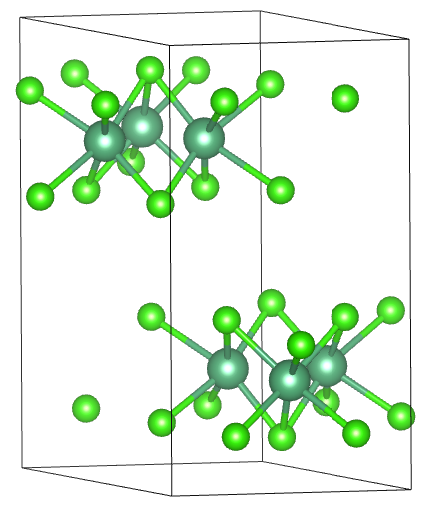
\includegraphics[width=0.8\linewidth]{figures/Nb3Cl8.png}
		\end{figure}
		\newpage
		\begin{itemize}
			\item \textbf{Component}: 2-class \textbf{Nb} $d$-orbitals
			\begin{enumerate}
				\item   $\left\{d_{z^2}\right\}$ 
				\item   $\left\{d_{x^2-y^2},d_{xy} ;\ d_{xz},d_{yz} \right\}$
			\end{enumerate}
			\item \textbf{Geometry}: Bilayer Kagome lattice of \textbf{Nb}.
		\end{itemize}
	\end{multicols}
\end{frame}

	
\begin{frame}{Hamiltonian}
	\begin{multicols}{2}
	\begin{align*}
		H =& -t\sum_{\langle i,j \rangle ,\sigma,\alpha}\left(c^\dagger_{i\sigma\alpha}c_{j\sigma\alpha} + \text{H.c.}\right) 
		\\ &- t'\sum_{\langle\langle i,j\rangle\rangle,\sigma,\alpha}\left(c^\dagger_{i\sigma\alpha}c_{j\sigma\alpha} + \text{H.c.}\right)
		\\ &+U\sum_{i,\alpha}n^d_{i\uparrow\alpha}n^d_{i\downarrow\alpha} 
		\\ &+ V\sum_{\langle i,j \rangle,\sigma,\alpha}n_{i\sigma\alpha}n_{j\sigma\alpha}
	\end{align*}
	\newpage
	\begin{itemize}
		\item \textbf{Extended Hubbard Model}
		\begin{enumerate}
			\item NN Hopping terms: $t$.
			\item NNN Hopping terms: $t'$.
			\item Onsite interaction: $U$.
			\item NN interaction: $U$.
		\end{enumerate}
		\item \textbf{Convention}: $c_{i\sigma\alpha}$ \\
		Annihilation operators of $d_\alpha$ orbitals at site $i$ with spin $\sigma$.\\
		$\alpha \in \left \{ z^2;x^2-y^2,xy;xz,yz \right \}$
	\end{itemize}
	\end{multicols}
\end{frame}

\begin{frame}{Hamiltonian}
	\begin{multicols}{2}
	\begin{align*}
		H =& -t_n\sum_{\langle i,j \rangle_n,\sigma,\alpha}\left(c^\dagger_{i\sigma\alpha}c_{j\sigma\alpha} + \text{H.c.}\right) 
		\\ &+V_n\sum_{\langle i,j \rangle_n,\alpha}n_{i\sigma\alpha}n_{j\sigma\alpha}
	\end{align*}
	\newpage
	\begin{itemize}
		\item \textbf{Extended Hubbard Model}
		\begin{enumerate}
			\item $n$ order neighbor hopping: $t_n$.
			\item $n$ order neighbor interaction: $V_n$.
		\end{enumerate}
		\item \textbf{Convention}: $c_{i\sigma\alpha}$ \\
		Annihilation operators of $d_\alpha$ orbitals at site $i$ with spin $\sigma$.\\
		$\alpha \in \left \{ z^2;x^2-y^2,xy;xz,yz \right \}$
	\end{itemize}
	\end{multicols}
\end{frame}
	
\begin{frame}{Parameters}
		\begin{itemize}
			\item Composite Triangular Lattice ($Lx\times 4\ \text{or}\ 6$) with \textbf{PBC}
			\begin{figure}[H]
				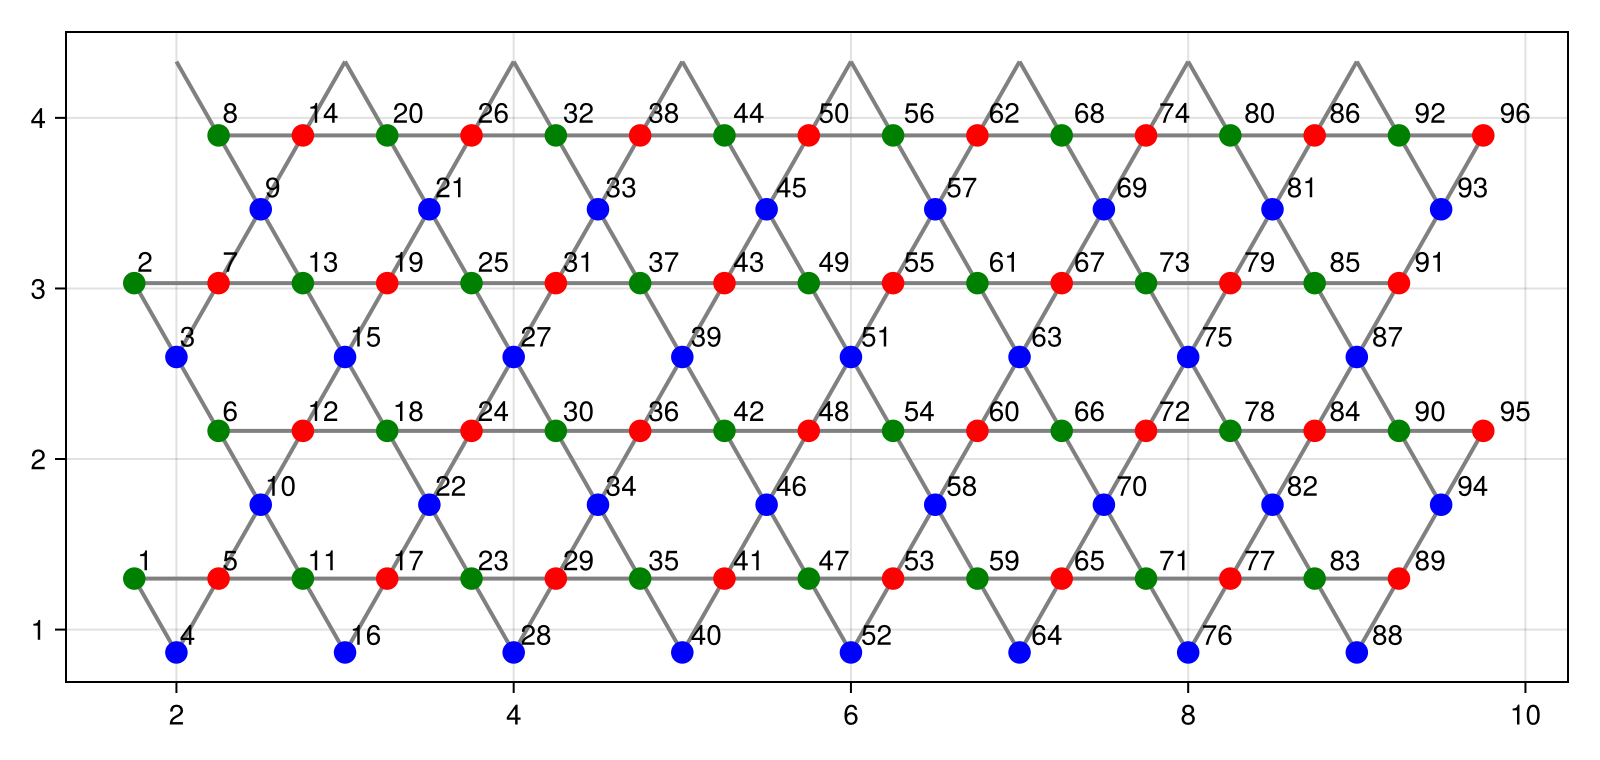
\includegraphics[width=0.8\linewidth]{figures/8x4Kagome.png}
			\end{figure}
			\item Parameters\\
			From DFT.
		\end{itemize}
\end{frame}

\begin{frame}{Observables}
	\begin{multicols}{2}
		\begin{figure}[H]
			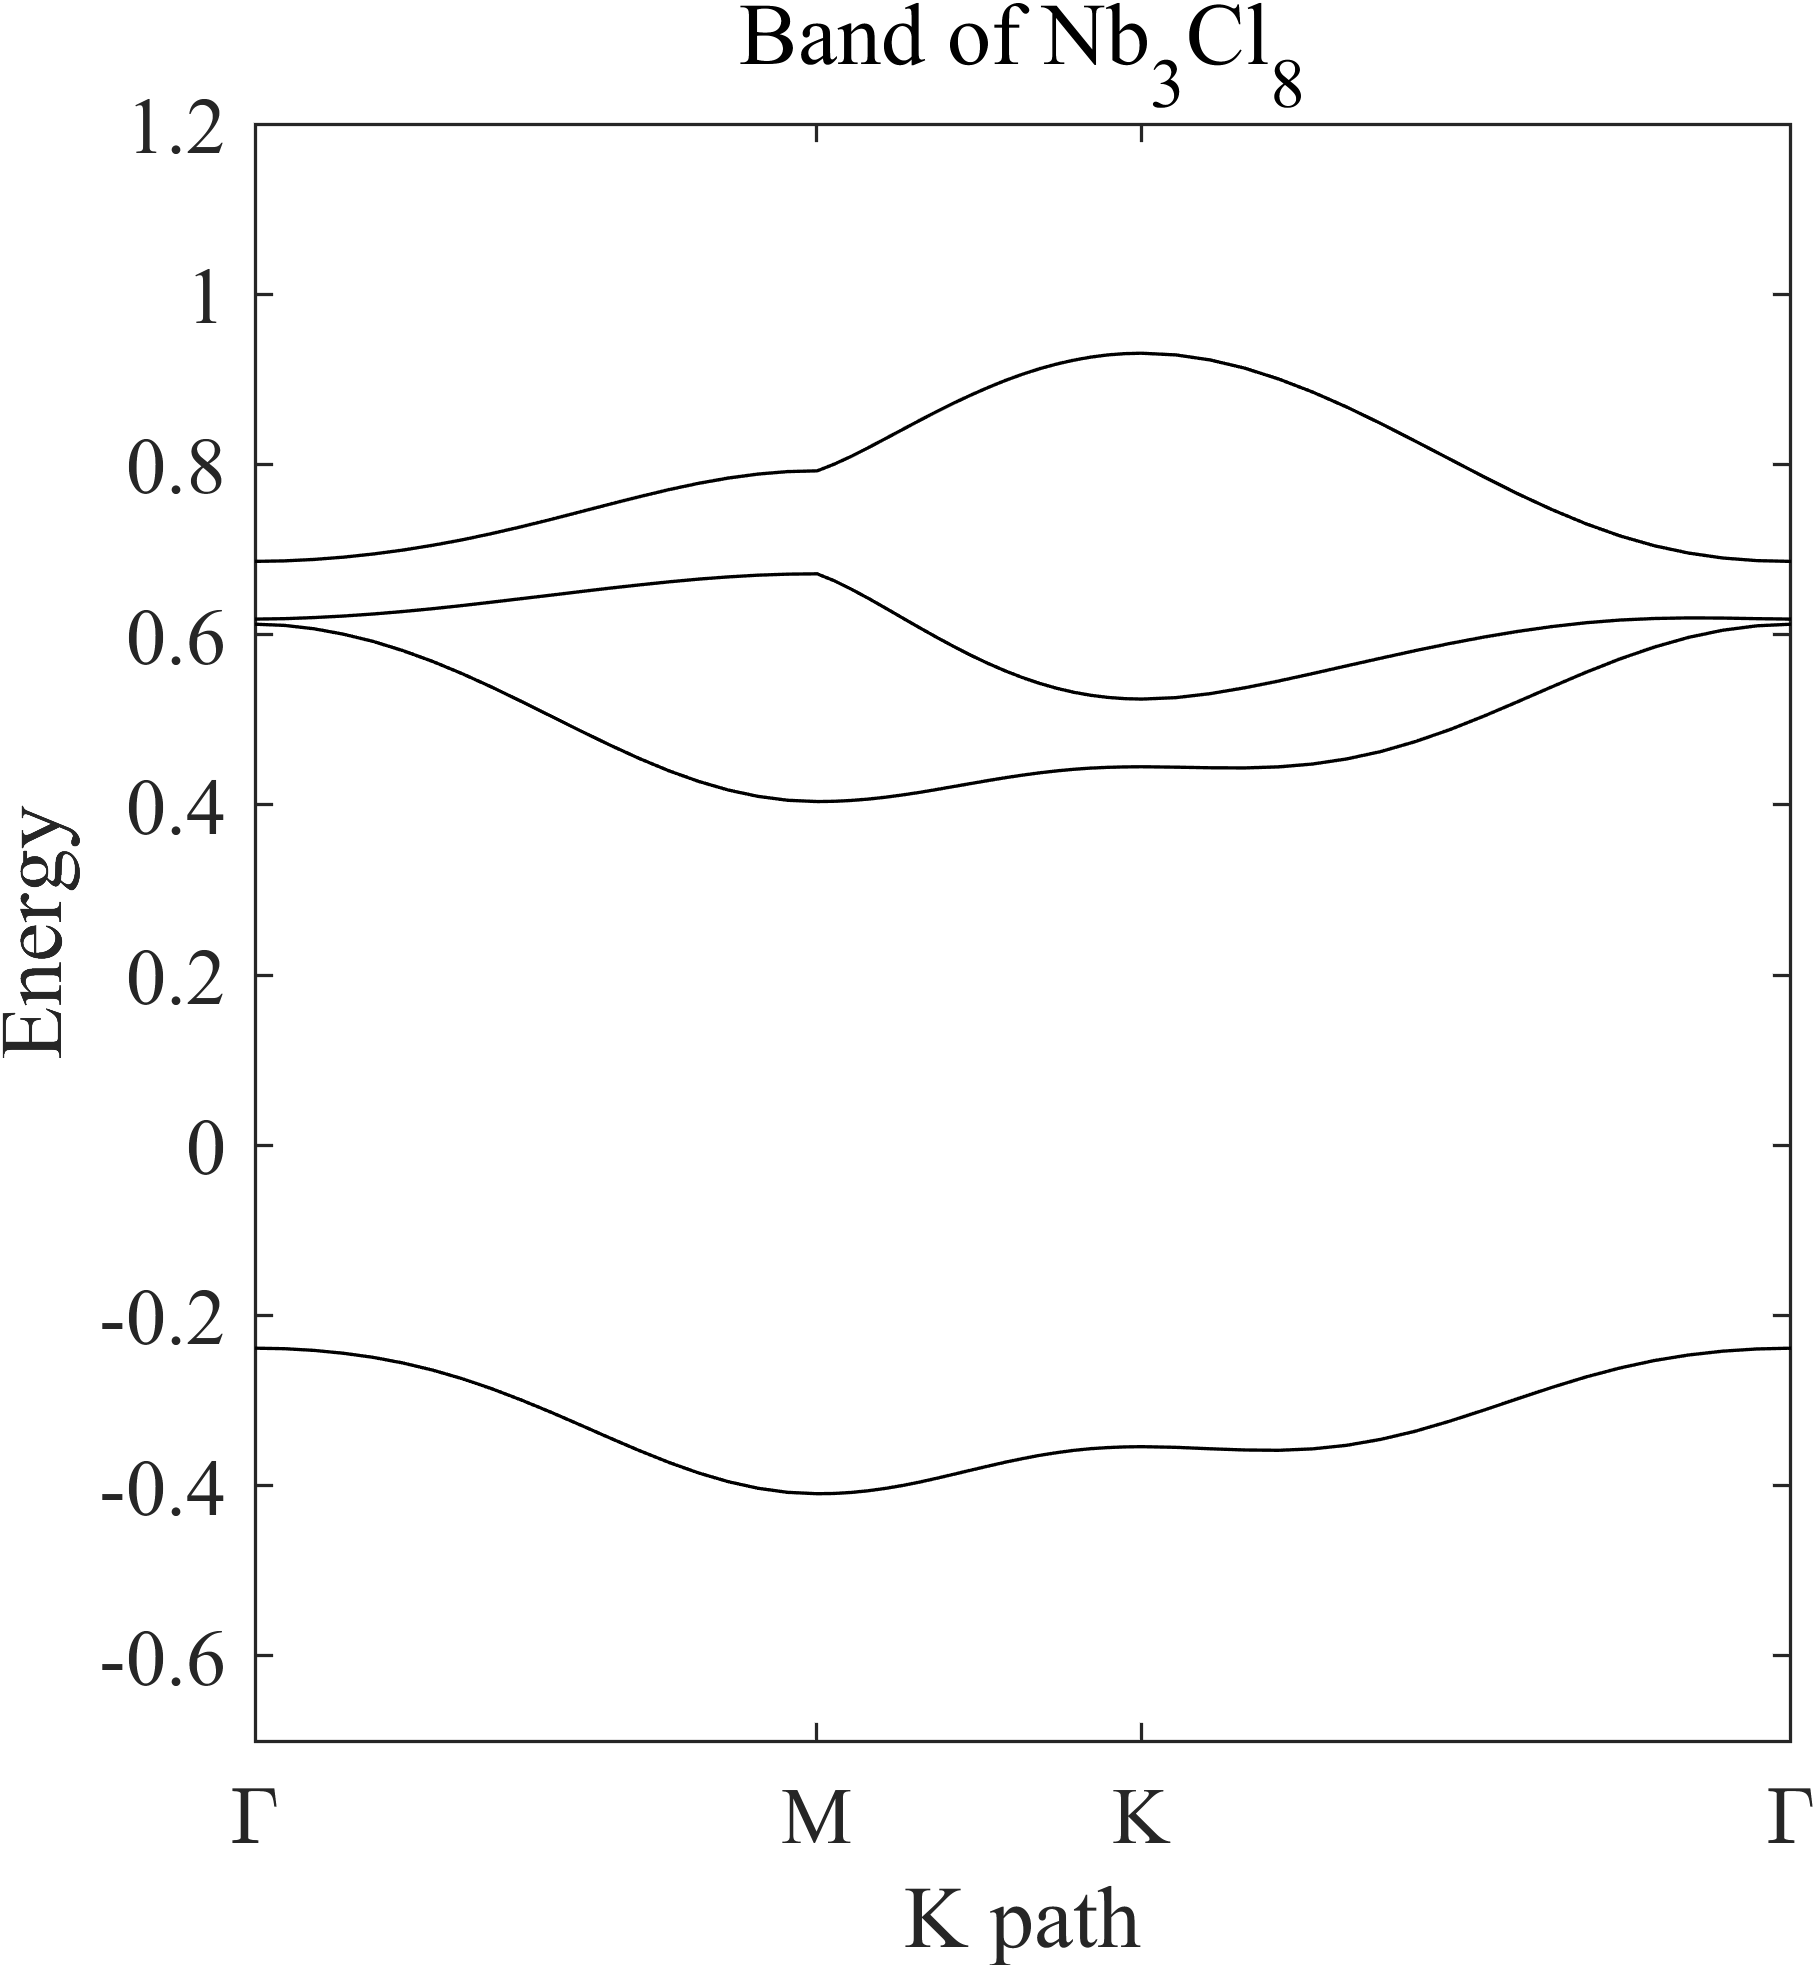
\includegraphics[width=1\linewidth]{figures/band.png}
		\end{figure}
		\newpage
		\begin{itemize}
			\item some observables
			\begin{equation*}
				\text{U1SU2: }n, n^d, \vb{S}_i\cdot \vb{S}_j,\quad \text{U1U1: }\cdots,S_z
			\end{equation*}
			\item Hamiltonian (Sing.Elec.Appr.)
			\begin{equation*}
				H = \sum_{\vb{k},n,\sigma}E_n(\vb{k})c^\dagger_{\vb{k}n\sigma}c_{\vb{k}n\sigma}
			\end{equation*}
			\item CB breation operator $c^\dagger_{\vb{k}c\sigma}$
			\begin{equation*}
				c^\dagger_{\vb{k}c\sigma}=\sum_{i,\alpha,\sigma}A_{c,i\alpha\sigma}(\vb{k})\mathrm{e}^{i\vb{k}\cdot \vb{R}_i}c^\dagger_{i\alpha\sigma}
			\end{equation*}
		\end{itemize}
	\end{multicols}
\end{frame}

\begin{frame}{Observables}
	\begin{multicols}{2}
		\begin{figure}[H]
			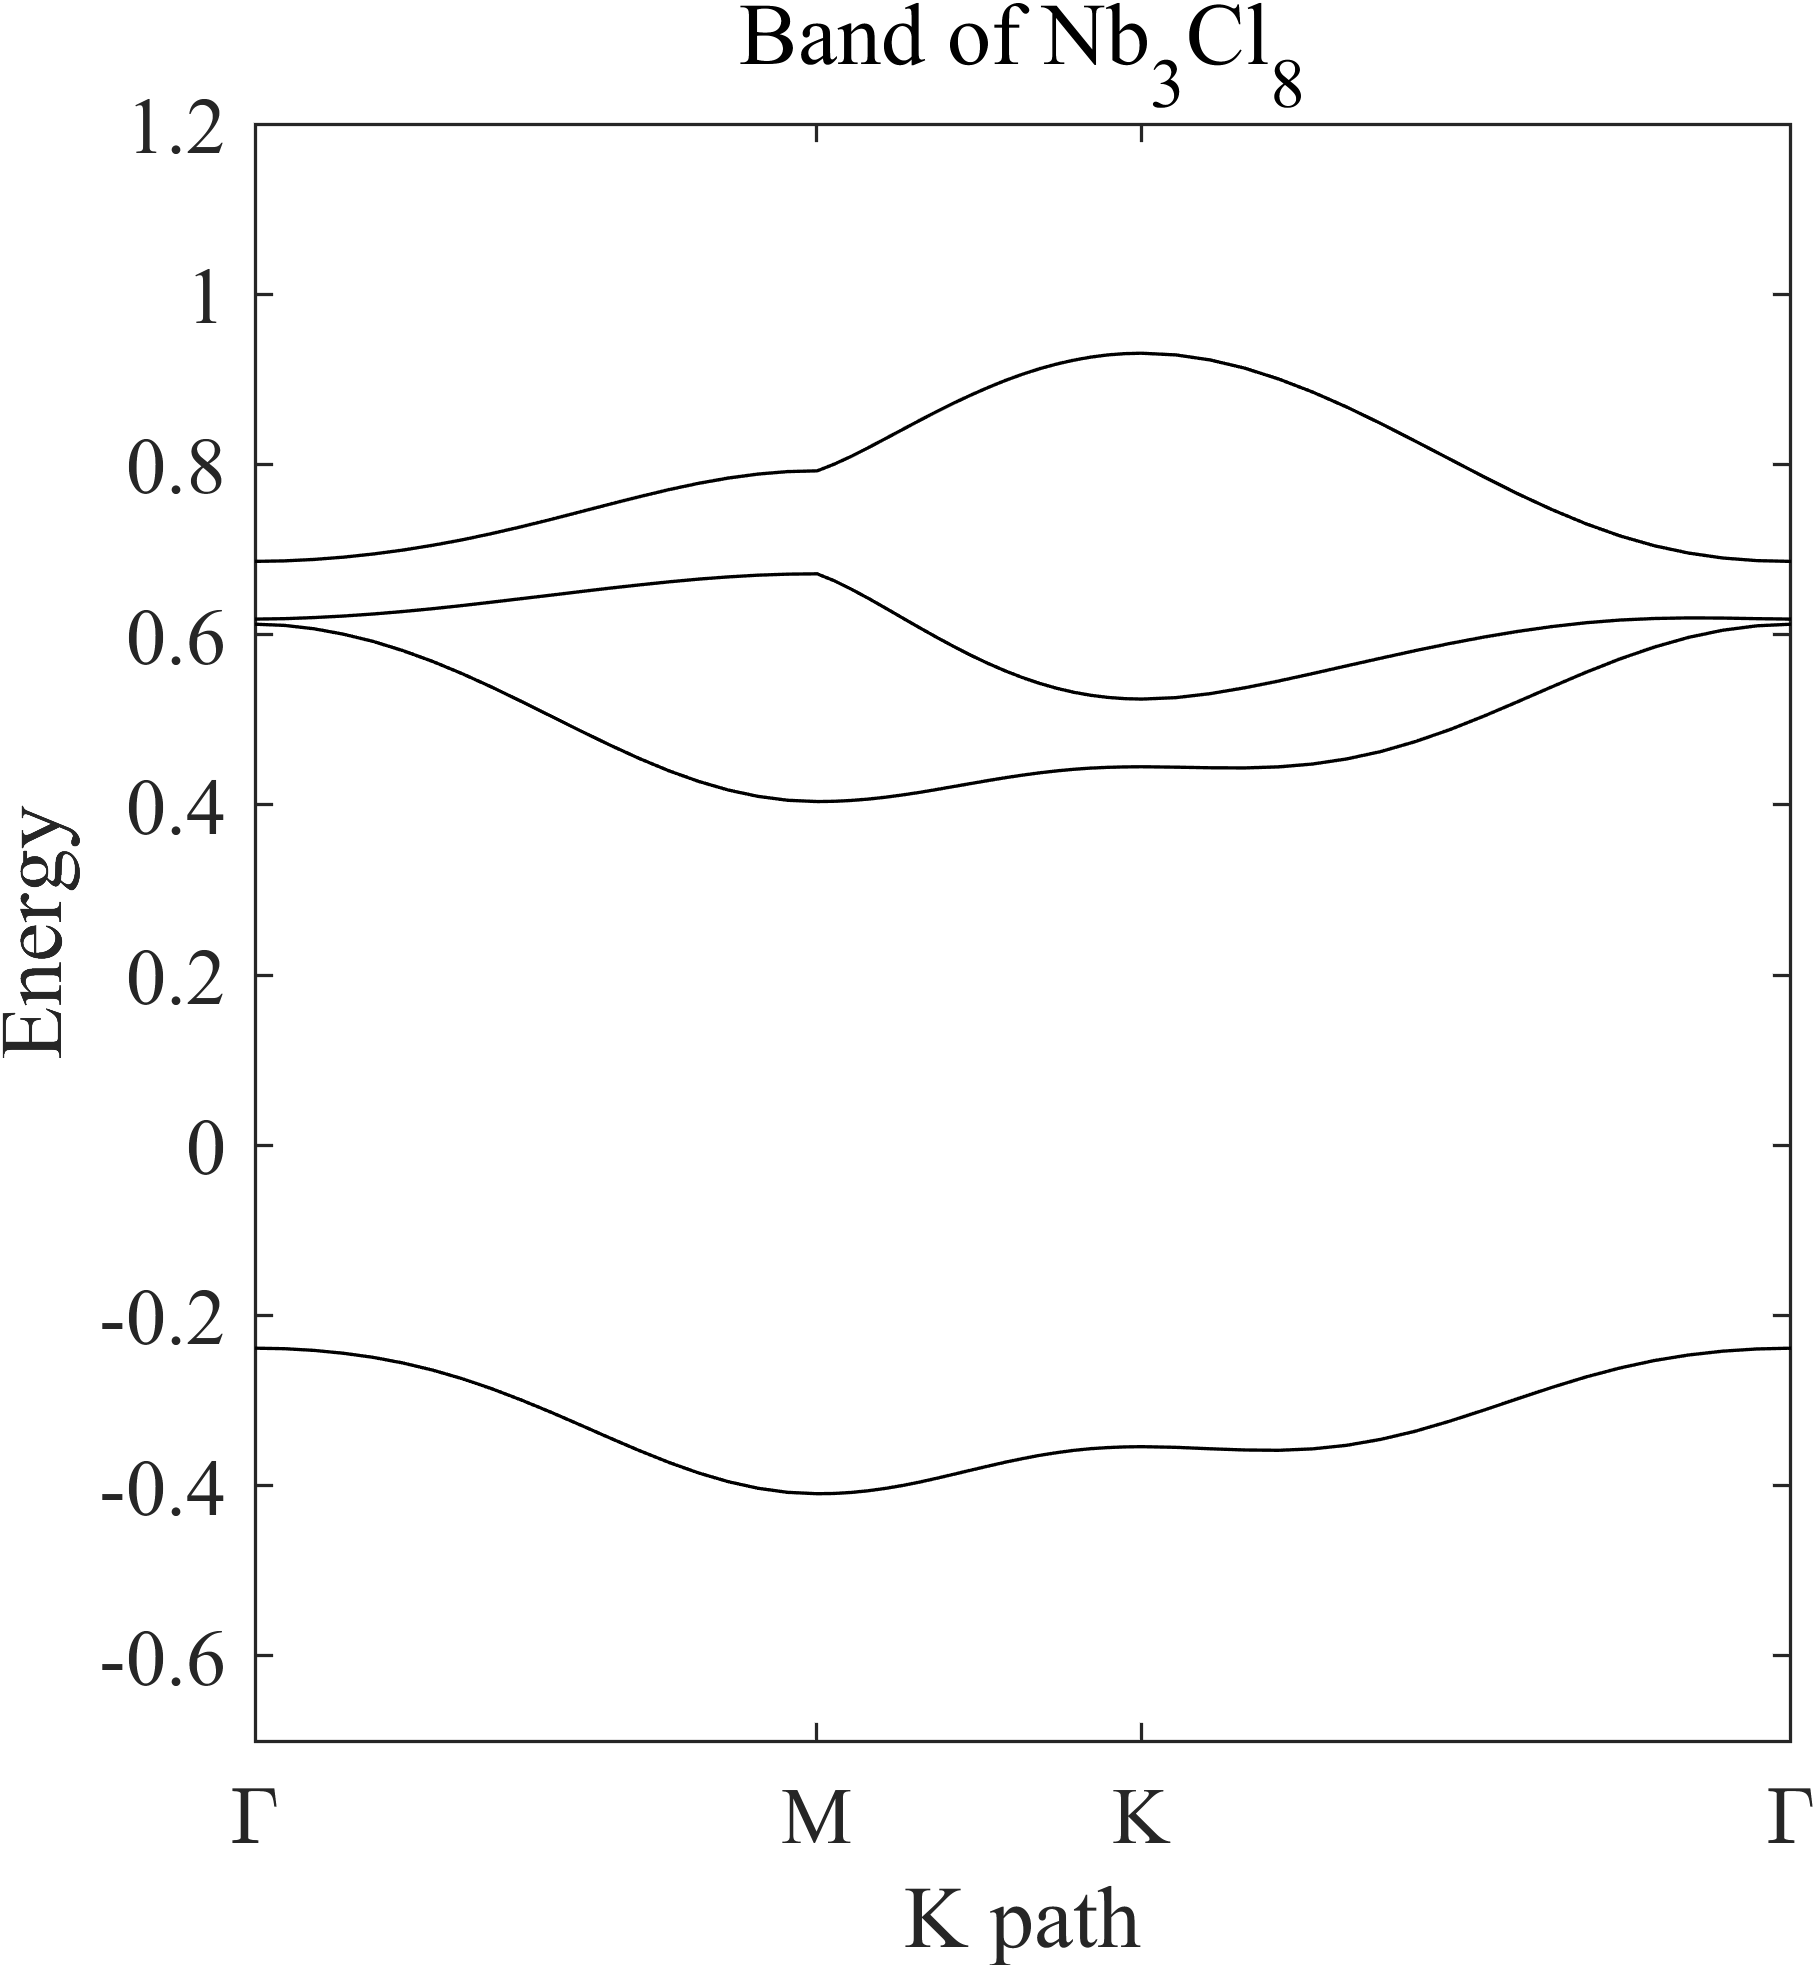
\includegraphics[width=1\linewidth]{figures/band.png}
		\end{figure}
		\newpage
		\begin{itemize}
			\item Exciton pairing operator $\Delta^\dagger_{\vb{q}\beta} $
			\begin{align*}
				%\Delta^\dagger_{m\vb{q}\sigma} = \sum_{\vb{k},\sigma}B_{c,i\alpha\sigma}(\vb{q})c^\dagger_{\vb{k+q}c\sigma}c_{\vb{k}v\sigma}
				\Delta^\dagger_{\vb{k+q,k}S} &=
				\\ &\frac{1}{\sqrt{2}}\left(c^\dagger_{\vb{k+q}c\uparrow}c_{\vb{k}v\downarrow}-c^\dagger_{\vb{k+q}c\downarrow}c_{\vb{k}v\uparrow}\right)\\
				\Delta^{\dagger,0}_{\vb{k+q,k}T} &= 
				\\ &\frac{1}{\sqrt{2}}\left(c^\dagger_{\vb{k+q}c\uparrow}c_{\vb{k}v\downarrow}+c^\dagger_{\vb{k+q}c\downarrow}c_{\vb{k}v\uparrow}\right)\\
				\Delta^{\dagger,1}_{\vb{k+q,k}T} &= c^\dagger_{\vb{k+q}c\uparrow}c_{\vb{k}v\uparrow}\\
				\Delta^{\dagger,-1}_{\vb{k+q,k}T} &= c^\dagger_{\vb{k+q}c\downarrow}c_{\vb{k}v\downarrow}
			\end{align*}
		\end{itemize}
	\end{multicols}
\end{frame}

\begin{frame}{Observables}
	\begin{multicols}{2}
		\begin{figure}[H]
			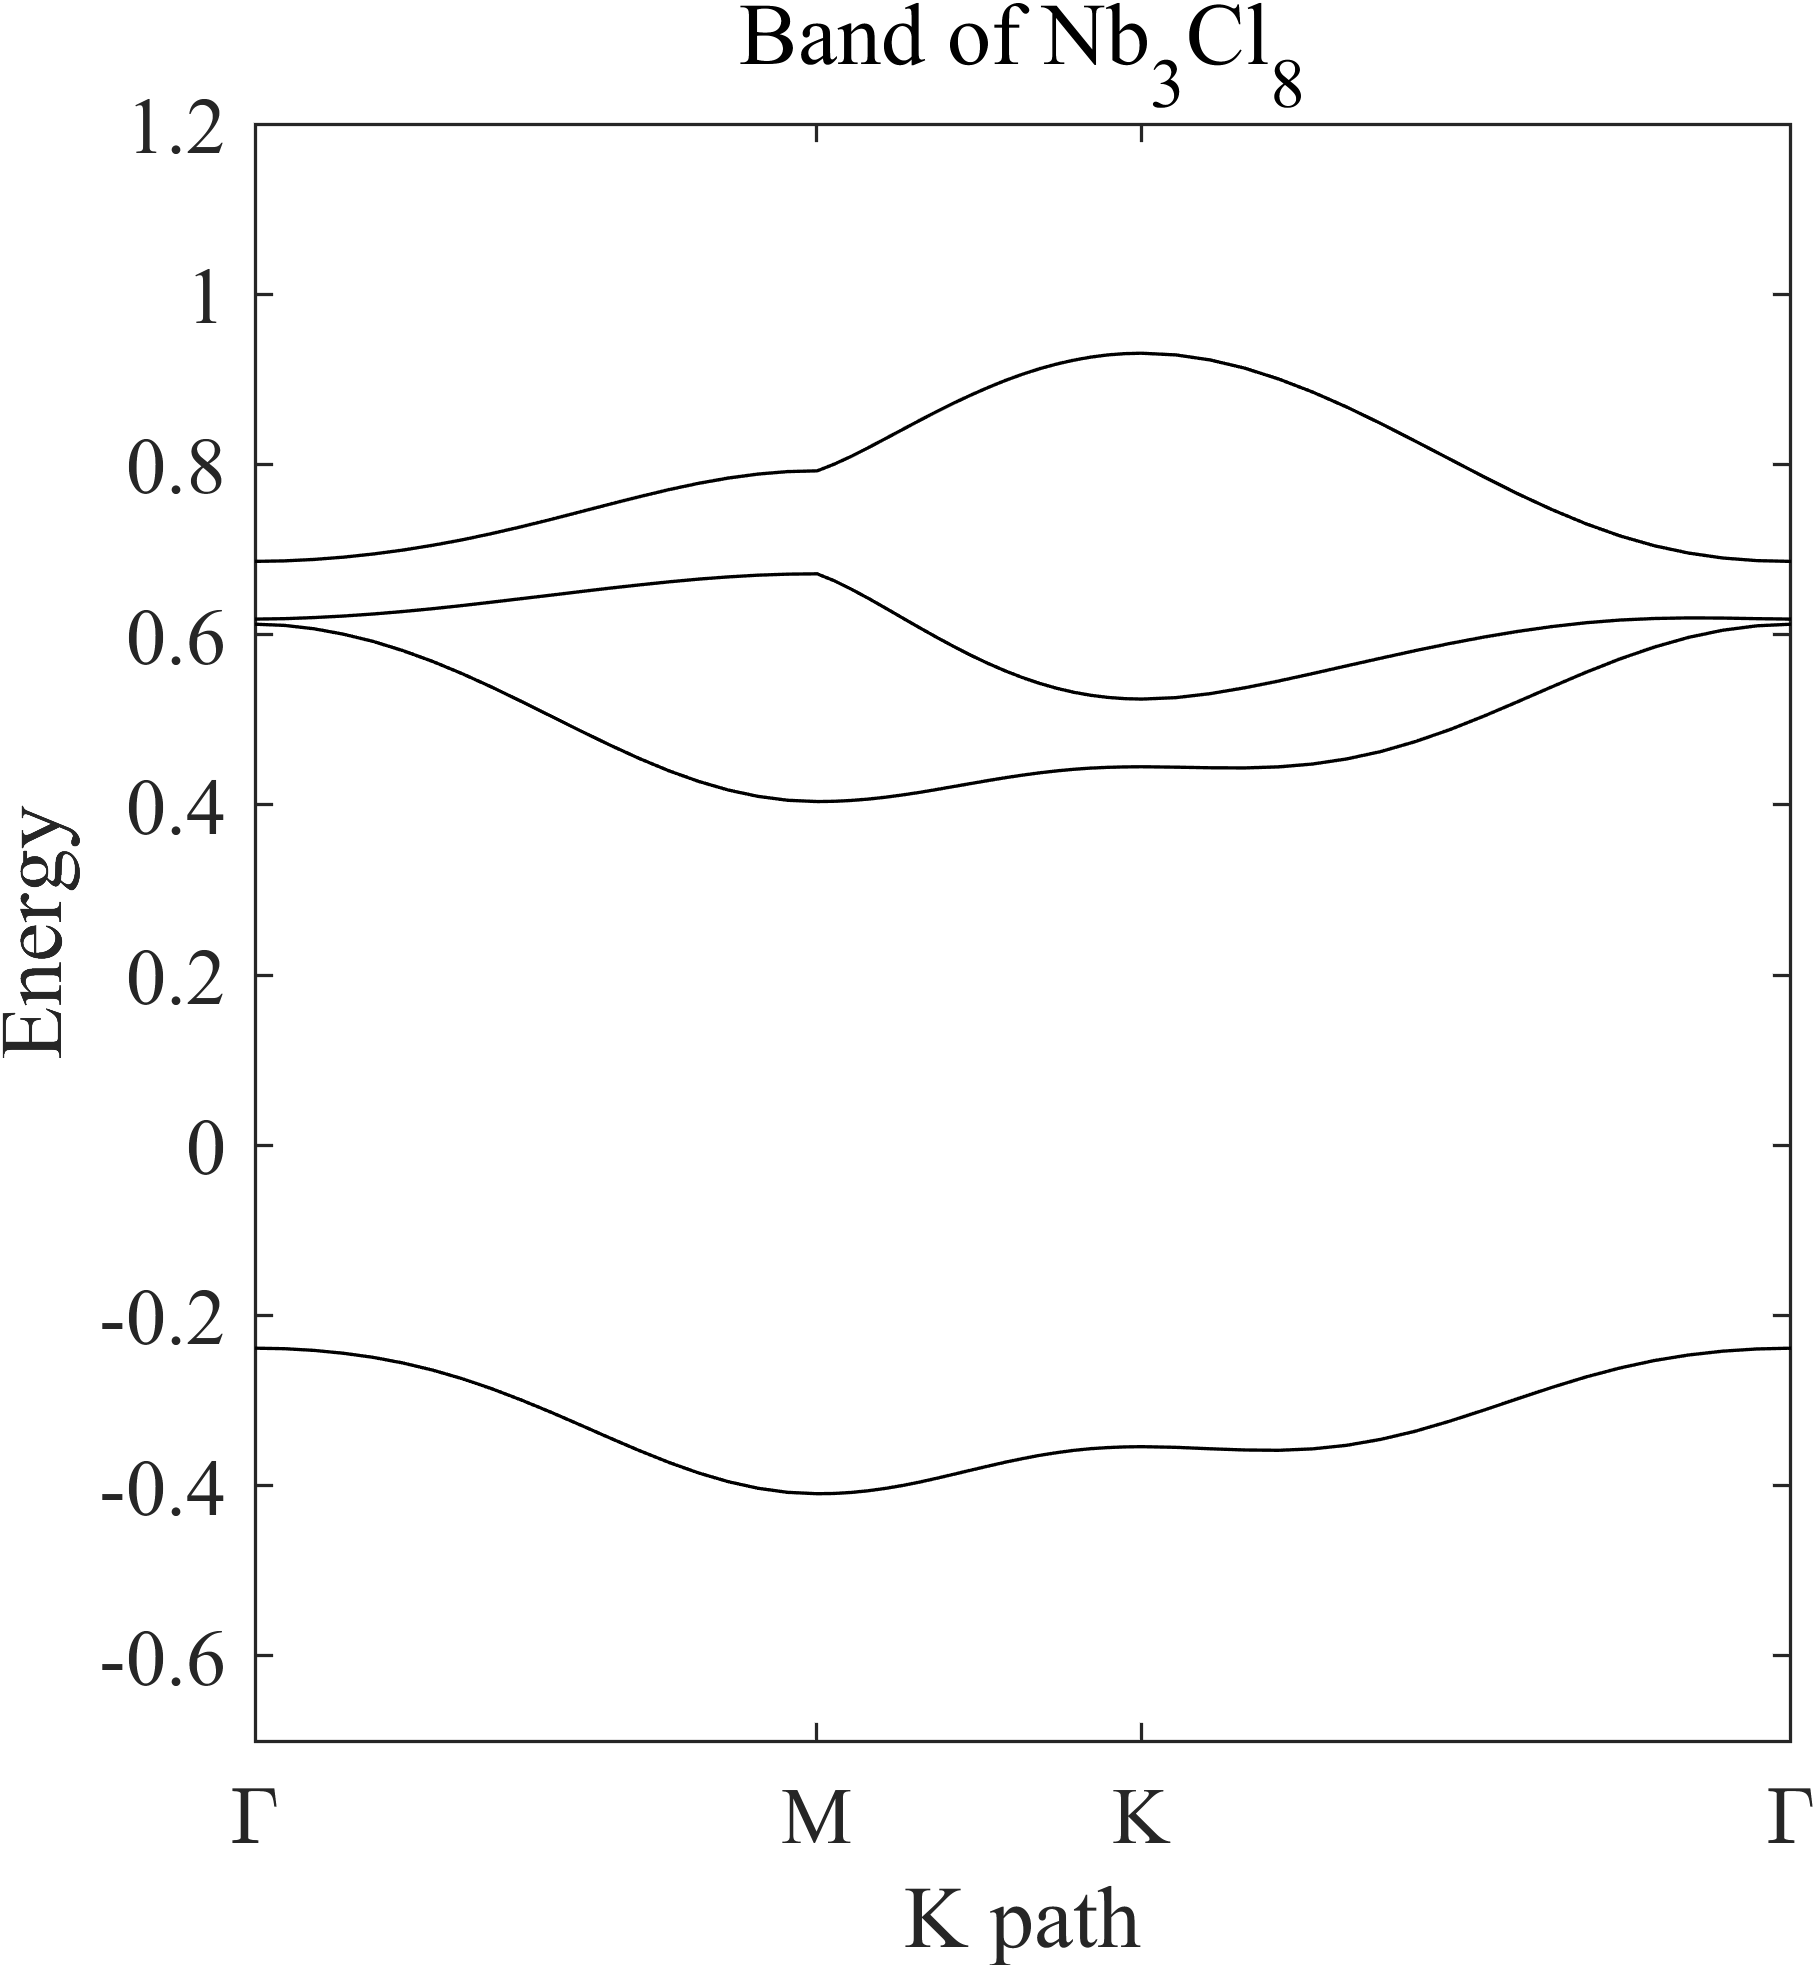
\includegraphics[width=1\linewidth]{figures/band.png}
		\end{figure}
		\newpage
		\begin{itemize}
			\item Properties $\Delta^\dagger_{\vb{k+q,k}\beta} $
			\begin{gather*}
				\expval{\Delta_{\vb{k+q,k}\beta}}{\Psi}=0\\
				\expval{\Delta^\dagger_{\vb{k,k'}\beta}\Delta_{\vb{\bar{k},\bar{k}'}\beta}}{\Psi}=?
			\end{gather*}
		\end{itemize}
	\end{multicols}
\end{frame}

\begin{frame}{Observables}
	\begin{definition}{Triplet-pairing density matrix}
		\begin{equation*}
			\rho_T^z(\vb{k,k'};\vb{\bar{k},\bar{k}'})=\expval{\Delta^{\dagger,z}_{\vb{k,k'}T}\Delta^{z}_{\vb{\bar{k},\bar{k}'}T}},\quad z = 0,1,-1
		\end{equation*}
	\end{definition}
	\begin{definition}{Singlet-pairing density matrix}
		\begin{equation*}
			\rho_S(\vb{k,k'};\vb{\bar{k},\bar{k}'})=\expval{\Delta^\dagger_{\vb{k,k'}S}\Delta_{\vb{\bar{k},\bar{k}'}S}}
		\end{equation*}
	\end{definition}
\end{frame}

\begin{frame}{Observables}
	\begin{definition}{$\vb{k}$ space pairing operator}
		\begin{equation*}
			\Delta _{\vb{k,k'}} = c^\dagger_{\vb{k}c}c_{\vb{k'}v}
			 = \sum_{s,l}c^\dagger_sc_l A_{c,i}^*(\vb{k})A_{v,j}(\vb{k'})\mathrm{e}^{i(\vb{k}\cdot \vb{R}_s-\vb{k'}\cdot \vb{R}_l)}
		\end{equation*}
	\end{definition}
	\begin{definition}{real space pairing operator}
		\begin{align*}
			\Delta _{\vb{i,j}} =& \int_{\vb{k,k'}}\Delta_{\vb{k,k'}}\mathrm{e}^{i(-\vb{k}\cdot \vb{R}_i+\vb{k'}\cdot \vb{R}_j)}\\
			=&\sum_{s,l}c^\dagger_sc_l\int_{\vb{k,k'}}A_{c,i}^*(\vb{k})A_{v,j}(\vb{k'})\mathrm{e}^{i(\vb{k}\cdot \vb{R}_s-\vb{k'}\cdot \vb{R}_l)}\mathrm{e}^{i(-\vb{k}\cdot \vb{R}_i+\vb{k'}\cdot \vb{R}_j)}
		\end{align*}
	\end{definition}
\end{frame}

\begin{frame}{PROBLEMS}
	\begin{itemize}
		\item real-space pairing operator do not exists
		\item Calculate 2-PBC system, which more close to a lattice system. 1-PBC for a stripe.
	\end{itemize}
\end{frame}


\end{document}
